%% -*- mode: LaTeX -*-
%%

%%%%%%%%%%%%%%%%%%%%%%%%%%%%%%%%%%%%%%%%%%%%%%%%%%%%%%%%%%%%%%%%%%%%%%%%%%%%%%%

\section{Related Work}
\label{sec:related}

The idea of measuring~\cite{pathloss, modelingand} radio frequency propagation as well as using propagation models to 
simulate~\cite{educationalsimulation} radio frequency propagation loss~\cite{directionalradio} is not a new idea. As we will see, there are multiple related works 
associated with this work, however, the overall idea is to compare Shout~\cite{shout} using a radio frequency tool, such as SPLAT!~\cite{splat}. 
SPLAT! is one of few open source radio frequency propagation modeling analysis tools. CloudRF~\cite{cloudrf} is another familiar radio 
propagation modeling tool that offers more in terms of cellular propagation models for mobile networks, as well as faster results due to its 
proprietary propagation engine. 

\begin{figure}
  \centering
  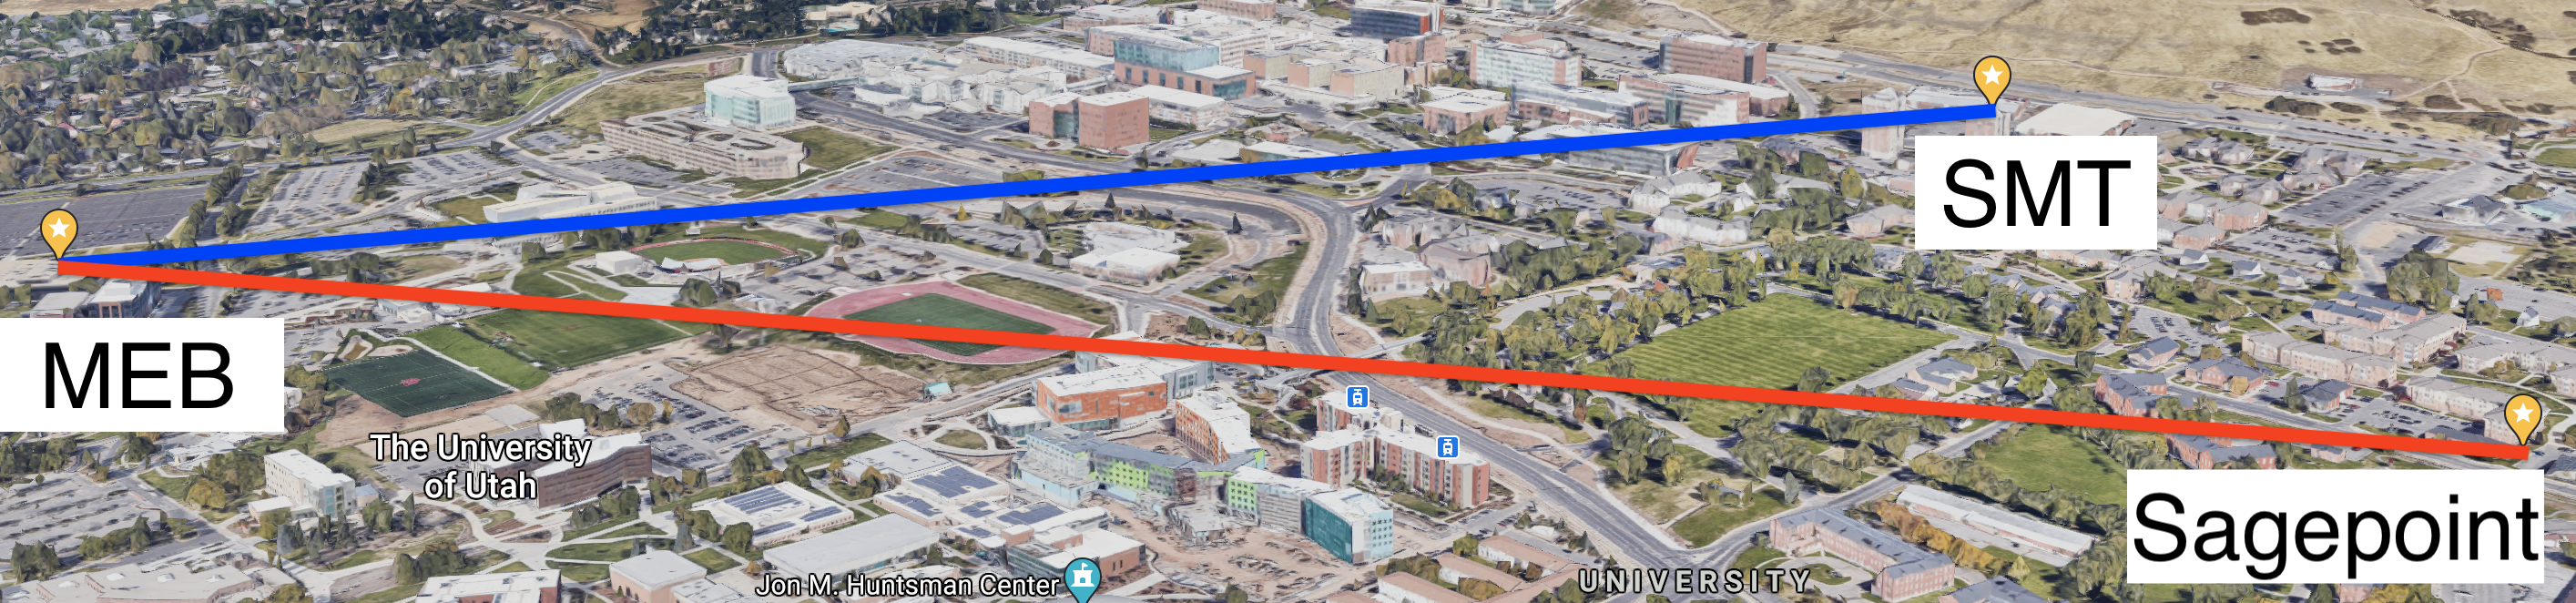
\includegraphics[width=0.9\columnwidth]{worst}
  \caption{MEB left with the red line leading to Sagepoint, while the blue leads to SMT.}
  \label{fig:worst}
\end{figure}

%
\subsubsection*{SPLAT!}
SPLAT! allows for propagation loss and terrain analysis for the electromagnetic spectrum between 20 MHz and 20 GHz. Our first 
example of SPLAT! is used in an architecture~\cite{hybridRF} that can be used for simulation and in-situ learning of the attenuation
of RF signals in the environment. SPLAT! is used to generate a prediction mean field for CU Mountain Research Station to determine
radio frequency propagation loss in the rocky terrain. 

Another study~\cite{comparisonof}, that similarly resembles ours, aims to compare accurate measurements taken by Rohde \& 
Schwarz portable spectrum analyzer and precision antennas for digital TV, with simulated results from multiple coverage prediction 
models like SPLAT!. However, SPLAT! in this study produces big differences compared with the real measurement results. This is 
due to SPLAT!'s inability to work properly in the line-of-sight mode as well as a lack of detailed terrain information. 

Digital Terrestrial Television (DTT) is degraded~\cite{dttperformance} due to the coexistence between LTE operating in the adjacent
frequency band. To study these results the authors of the paper used SPLAT! to produce a DTT system model. To produce such a model
they took into account earth conductivity, atmospheric bending constant, antenna polarization, relative permittivity, and antenna height above
the ground.
%
\subsubsection*{CloudRF}
Long Range (LoRa) is a low-power wide-area networking protocol that is designed to connect Internet of Things (IoT) devices to the 
internet in regional, national or global networks. Deployment of LoRa access points requires taking into consideration the spatial 
distribution of clients, and radio signal propagation. A heuristic algorithm~\cite{heuristicalgorithm} was designed for gateway location
selection for LoRa networks. CloudRF was used to estimate the coverage of LoRa gateways on the map allowing the algorithm to
decide if the placement of access nodes are at the best place they could be. 

Similarly, a simulation~\cite{asimulation} was done to replace the Peruvian Navy's Supervisory Control and Data Acquisition (SCADA) 
system with an IoT-based solution using LoRaWAN. SCADA is a system to monitor and control remote meteorological and luminous 
stations. Path loss calculations between stations were made using the Okumura-Hata radio propagation model. The results were then 
validated using CloudRF. Results conclude that the LoRaWAN system is superior to the currently used SCADA system. 
%
\subsubsection*{Propagation Models}
Propagation models are designed in order to give acceptable accuracy level and computational complexity. Ray tracing~\cite{modelingand} 
is one example of deterministic models. Ray tracing is a method for calculating wave propagation through the use of repeatedly advanced
narrow beams through a medium by discrete amounts. Through the use of Maxwell's equations ray tracing provides valid wave propagation
measurements.

A comparison~\cite{comparisonofempirical} of three path loss models for fixed wireless access systems was done. The comparison
measurements were taken at 3.5 GHz in Cambridge, UK and their applicability was validated in three environments: rural, suburban,
and urban environments. Specifically, three empirical models the Stanford University Interim (SUI), the COST-231 Hata, and the ECC-33 
models were chosen for this comparison. The results show that ECC-33 model shows the best results, especially in urban environments.
While for the general case the COST-231 Hata and SUI models highly over predict the path loss in all the environments. 

%%%%%%%%%%%%%%%%%%%%%%%%%%%%%%%%%%%%%%%%%%%%%%%%%%%%%%%%%%%%%%%%%%%%%%%%%%%%%%%

%% End of file.